%%%%%%%%%%%%%%%%%%%%%%%%%%%%%%%%%%%%%%%%%%%%%%%%%%%%%%%%%%%%%%%%%%%
%                                                                 %
%                            CHAPTER THREE                        %
%                                                                 %
%%%%%%%%%%%%%%%%%%%%%%%%%%%%%%%%%%%%%%%%%%%%%%%%%%%%%%%%%%%%%%%%%%%

\chapter{METHODOLOGY}\label{ch:model}

\section{Introduction}

A versioning data model needs to address a variety of needs not met by provenance models.
The model must contain a mechanism to convey how changes to parts of an object contribute to that object's transition into a new version.
The fundamental operations---\textbf{add}, \textbf{invalidate}, and \textbf{modify}---are used by the model to capture change in a more detailed manner.
These details provide a mechanism to measure change between versions with better clarity than current methods.

\section{Model Objects}

The versioning model incorporates three kinds of objects: \textbf{versions}, \textbf{attributes}, and \textbf{changes}.
A \textbf{version} object represents the items being compared such as a book or spreadsheet.
In PROV, a \textbf{version} would likely correspond with the \textit{prov:Entity} involved in a \textit{prov:wasRevisionOf} property.
The \textbf{attribute} object refers to specific parts which make up a \textbf{version}.
\textbf{Attributes} could be lines in a book or columns in a spreadsheet.
Including \textbf{attributes} addresses the lack of detail involved in a \textit{prov:wasRevisionOf} or \textit{pav:previousVersion}.
The relationship between \textbf{versions} and \textbf{attributes} captures the influence that changes in the underlying part will have on the overarching \textbf{version}.
Because the model refers to specific parts of a \textbf{version}, the \textbf{version} concept corresponds most closely with a FRBR \textbf{manifestation} rather than an \textbf{expression}.
The presence or absence of an \textbf{attribute} is used to determine the kind of \textbf{change} which occurs to the \textbf{attribute} between \textbf{versions}.
\textbf{Changes} are used to link together \textbf{attributes} from different \textbf{versions}.
The \textbf{change} captures a difference between the old \textbf{version} state and the new \textbf{version} state.
While the \textbf{change} object greatly resembles a PROV qualified property, its form can change depending on the kind of \textbf{change}, like a \textit{schema:UpdateAction}.

\subsection{Left-hand Right-hand Convention}

In the following diagrams and figures, the original or base version and its attributes will be placed on the left-hand side and the new version will be placed on the right-hand side with its attributes.
References to the versions as previous and next are avoided since sequencing may not play a major role in distinguishing versions.
Scientific data in large repositories often track sequential releases of data, but a book may have different versions distinguished by printed language.
To recognize this distinction, objects will be referred to as the left-hand \textbf{version} or left-hand \textbf{attribute} when they are not sequentially or temporally related.

\section{Model Changes}

The model bases \textbf{changes} around the three core versioning operations because their commonality across systems provides a fundamental basis for comparisons.
\textbf{Additions} occur when an \textbf{attribute} appears only in the right-hand \textbf{version}.
When an \textbf{attribute} only shows up in the left-hand \textbf{version}, the model captures this as an \textbf{invalidation}.
Finally, a \textbf{modification} change has \textbf{attributes} in both the left and right-hand \textbf{versions}, but it only connects two \textbf{attributes} if their values are different.
These three combinations cover the possible situations within the model.

\begin{figure}
	\centering
	\vspace{0.0in} % normally the command here would be \includegraphics
	%	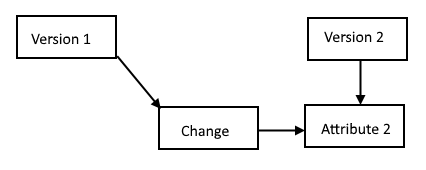
\includegraphics{figures/Addition.png}
	\begin{tikzpicture}[every node/.style={draw, rectangle}]
	\begin{scope}[node distance=20mm and 20mm]
	\node (c) [scale=1.25] at (1,0) {Change M};
	\node (1) [above left=of c, scale=1.25] {Version 1};
	\node (2) [above right=of c, scale=1.25] {Version 2};
	\node (a1) [below =of 1, scale=1.25] {Attribute 1};
	\node (a2) [below =of 2, scale=1.25] {Attribute 2};
	
	\draw [line width=2pt,->] (a1) -- (c);
	\draw [line width=2pt,->] (c) -- (a2);
	\draw [line width=2pt, ->] (1) -- (a1);
	\draw [line width=2pt, ->] (2) -- (a2);
	\end{scope}
	\end{tikzpicture}
	\caption{Model of the relationships between Versions 1 and 2 when modifying Attribute 1 from Version 1 as a result of Change M, resulting in Attribute 2 from Version 2}
	\label{ModificationFig}  % the \label command comes AFTER the caption
\end{figure}

\subsection{Modification}

The \textbf{modification} relation occurs when an \textbf{attribute} appears in both \textbf{versions} and their values are different.
In Figure \ref{ModificationFig}, a \textbf{modification} is captured between two versions.
Each \textbf{version} has an \textbf{attribute}, Attribute 1 and Attribute 2, respectively.
Finally, a \textbf{change} object connects the two \textbf{attributes}, denoting that the values described by the attribute are different.

The specific values pertaining to Attribute 1 and Attribute 2 are not captured by the model because acknowledging that a difference exists is more important.
Extending the model to properly communicate the significance of a modification for a wide variety of domains would require sizable domain knowledge and would be outside the scope for this project.
In addition, the model would essentially begin storing a copy of the data set, leading to space and redundancy concerns.

\subsection{Addition}

In Figure \ref{AdditionFig}, the \textbf{addition} model differs from the \textbf{modification} construction by the absence of Attribute 1.
\begin{figure}
	\centering
	\vspace{0.0in} % normally the command here would be \includegraphics
	%	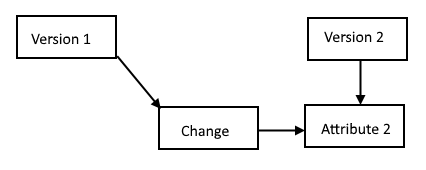
\includegraphics{figures/Addition.png}
	\begin{tikzpicture}[every node/.style={draw, rectangle}]
	\begin{scope}[node distance=20mm and 20mm]
	\node (c) [scale=1.25] at (1,0) {Change A};
	\node (1) [above left=of c, scale=1.25] {Version 1};
	\node (2) [above right=of c, scale=1.25] {Version 2};
	\node (a) [below =of 2, scale=1.25] {Attribute 2};
	
	\draw [line width=2pt,->] (1) -- (c);
	\draw [line width=2pt,->] (c) -- (a);
	\draw [line width=2pt, ->] (2) -- (a);
	\end{scope}
	\end{tikzpicture}
	\caption{Model of the relationships between Versions 1 and 2 when adding an Attribute 2 to Version 2 as a result of Change A}
	\label{AdditionFig}  % the \label command comes AFTER the caption
\end{figure}
The absence creates a disconnect between ``Version 1" and ``Change A".
A property is used to create a path between the two \textbf{attributes} to indicate the contribution of  ``Version 1" to the change's lineage.
The path does not show that ``Version 1" informs or creates ``Attribute 2", while that may be true.
The construction was also chosen to create a symmetric orientation with the \textbf{invalidation} change.


\subsection{Invalidation}

The \textit{invalidation} model has a missing \textbf{attribute} on the right-hand side of the relation, contrary to the \textbf{addition} construction.
As a result of the invalidation, an attribute no longer exists in the right-hand \textbf{version}.
As seen in Figure \ref{InvalidationFig}, the invalidation change concept matches to the Version 2 object.
\begin{figure}
	\centering
	\vspace{0.0in} % normally the command here would be \includegraphics
	%	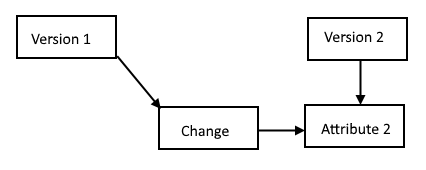
\includegraphics{figures/Addition.png}
	\begin{tikzpicture}[every node/.style={draw, rectangle}]
	\begin{scope}[node distance=15mm and 20mm]
	\node (c) [scale=1.25] at (1,0) {Change I};
	\node (1) [above left=of c, scale=1.25] {Version 1};
	\node (2) [above right=of c, scale=1.25] {Version 2};
	\node (a) [below =of 1, scale=1.25] {Attribute 1};
	
	\draw [line width=2pt,->] (a) -- (c);
	\draw [line width=2pt,->] (c) -- (2);
	\draw [line width=2pt, ->] (1) -- (a);
	\end{scope}
	\end{tikzpicture}
	\caption{Model of the relationships between Versions 1 and 2 when invalidating Attribute 1 from Version 1 as a result of Change I}
	\label{InvalidationFig}  % the \label command comes AFTER the caption
\end{figure}
Just like in \textbf{addition} model, this construction maintains a link between the two \textbf{version} objects.
In this case, it makes more conceptual sense, however, because ``Version 2" invalidates ``Attribute 1" by omitting it.


\section{Summary}

The versioning model provides a method to capture change information in greater detail than current provenance models.
The inclusion of \textbf{versions} and \textbf{attributes} into the model connect changing items with the objects they influence.
The \textbf{changes} create a ladder-like structure to connect together \textbf{version} objects in greater detail.
Each rung of the ladder can not only be counted, but also grouped into types of change according to the respective operation.
The method of instantiating a versioning graph will be covered in Chapter \ref{ch:implement}.